\documentclass[12pt, a4paper, openany]{report}

\def\VersionRapport{1.0}

\usepackage[utf8]{inputenc} % un package
\usepackage[T1]{fontenc}      % un second package
\usepackage[francais]{babel}  % un troisième package
\usepackage{layout}
\usepackage[top=2.7cm, bottom=2.5cm, left=3.5cm, right=3cm]{geometry}
\usepackage{setspace}

\frenchbsetup{StandardLists=true} % à inclure si on utilise \usepackage[french]{babel}
%\usepackage{enumitem}
\usepackage[shortlabels]{enumitem}
\usepackage{amssymb}

\usepackage{color}
\usepackage{listings}
\definecolor{dkgreen}{rgb}{0,0.6,0}
\definecolor{gray}{rgb}{0.5,0.5,0.5}
\definecolor{mauve}{rgb}{0.58,0,0.82}

\lstset{frame=tb,
  language=Java,
  aboveskip=3mm,
  belowskip=3mm,
  showstringspaces=false,
  columns=flexible,
  basicstyle={\small\ttfamily},
  numbers=none,
  numberstyle=\tiny\color{gray},
  keywordstyle=\color{blue},
  commentstyle=\color{dkgreen},
  stringstyle=\color{mauve},
  breaklines=true,
  breakatwhitespace=true,
  tabsize=3
}

\usepackage{multirow} % pour les tableaux
\usepackage[table]{xcolor} % pour les tableaux

\usepackage{verbatim}
\usepackage{moreverb}
\usepackage{url}
\usepackage{pst-all}
\usepackage{eso-pic,graphicx}
\usepackage{caption} 
\usepackage[colorlinks=true,urlcolor=blue,linkcolor=red]{hyperref}
\usepackage{array}
\usepackage[toc,page]{appendix}
\usepackage[off]{auto-pst-pdf}
\usepackage{hyperref} % pour le sommaire table des matières
\AddThinSpaceBeforeFootnotes % à insérer si on utilise \usepackage[french]{babel}
\FrenchFootnotes % à insérer si on utilise \usepackage[french]{babel}
\usepackage{fancyhdr}
\pagestyle{headings}
\usepackage{pifont}  %pour les puces
\usepackage{amsmath} %pour les puces

\usepackage{verbatim} % pour le code en annexe 

%%%%%%%colones 
\newcolumntype{R}[1]{>{\raggedleft\arraybackslash }b{#1}}
\newcolumntype{L}[1]{>{\raggedright\arraybackslash }b{#1}}
\newcolumntype{C}[1]{>{\centering\arraybackslash }b{#1}}
%%%%%%% 

\renewcommand{\appendixpagename}{Annexes}
\renewcommand{\appendixtocname}{Annexes}

\title{Theme: Compte Rendu Système Linéaire à Temps Continu 1}
\author{REBOUT \bsc{Mehenna}}
\author{BOUYOUCEF \bsc{Farid}}
\date{2018-2019}



%new
\newcommand{\HRule}{\rule{\linewidth}{0.5mm}}


\begin{document}

%\selectlanguage{francais}
\pagenumbering{arabic} 

\makeatletter
  \begin{titlepage}
  

  \begin{sffamily}
   \begin{center}

    % Upper part of the page. The '~' is needed because \\
    % only works if a paragraph has started.
    
\includegraphics[scale=0.5]{Logo_UT3.jpg}~\\[1.5cm]

    \textsc{\LARGE Master 1 EEA ISTR/RODECO  }\\[2cm]

    \textsc{\Large Compte Rendu  Système Linéaire à Temps Continu 1}\\[1.5cm]

    % Title
    \HRule \\[0.4cm] % saut de ligne
    { \huge \bfseries TP 1 Pendule\\[0.4cm] }

    \HRule \\[1cm]   % sous de ligne 
    
\includegraphics[scale=0.1]{logomaster.jpg}
    \\[1cm]

    % Author and supervisor
    \begin{minipage}{0.4\textwidth}
      \begin{flushleft} \large
         \textsc{\emph {Réalisés par:} \\REBOUT Mehenna}\\
         \textsc{BOUYOUCEF Farid}   
          \newline
          Promotion 2018-2019 \\
      \end{flushleft}
    \end{minipage}
    \begin{minipage}{0.4\textwidth}
      \begin{flushright} \large
        \emph{Tuteur :}  \textsc{M DUROLA}\\
        \emph{Responsable de la Formation:} \textsc{M GOUAISBAUT}
      \end{flushright}
    \end{minipage}

    \vfill

    % Bottom of the page
    {\large Octobre 2018}

  \end{center}
  \end{sffamily}      
          
  \end{titlepage}
  
\makeatother




   
%*********************** somaire **************
\renewcommand{\contentsname}{Sommaire}
\tableofcontents
%*********************** listes des figures **************
\listoffigures
%*********************** listes des tableaux **************
\listoftables
 
 
 
 %*********************** INTRODUCTION **************
\chapter*{Introduction}Dans ce TP on va réaliser un asservissement de position ,on va utiliser pour cette manipulation la platine voir   la Figure 1.1.
\addcontentsline{toc}{chapter}{Introduction}

\begin{center}
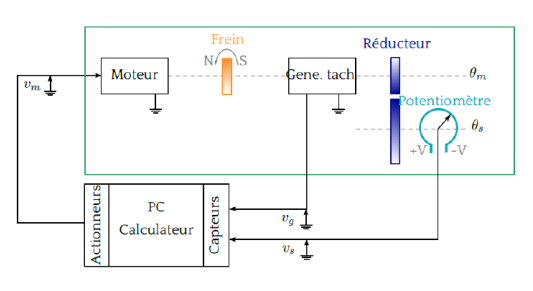
\includegraphics[scale=0.5]{fiiig1.png}
\captionof{figure}{\textit{Asservissement de position par calculateur}}
\label{fig1} 
\end{center}

Les valeurs numériques des coefficients connus sont:\\

 $K_e=10(V.tr^-1)$	 \hfill		$K_s=10(V.tr^-1)$	\hfill		$Kg=0.105(V.s.tr^-1)$ 
  \chapter{ PRÉLIMINAIRE DU PROCÉDÉ}
   \section{Représentation et analyse de ensemble (moteur, réducteur, potentiomètre, génératrice        tachymétrique) pour le système $ {S_V}_m \rightarrow V_S$ }
 

\begin{center}
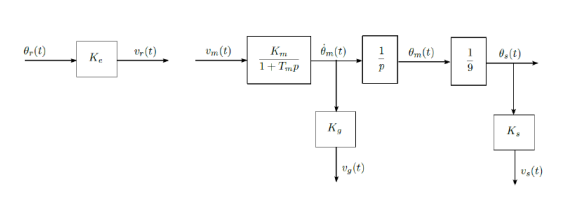
\includegraphics[scale=0.5]{fiiig2.png}
\captionof{figure}{\textit{ Eléments de la platine "asservissement de positon"}}
\label{fig1} 
\end{center}

On considère le système en boucle ouverte l’entrée du système on boucle ouvert est $V_m(t)$ et la sortie mesurée $V_s(t)$, que l’on note  par $ {S_V}_m \rightarrow V_S$.


\subsection{la représentation d’état de ce système, lorsque son vecteur d’état est défni par:}


\begin{equation}
x(t)={(x_1(t),x_2(t))}^T={(V_s(t),V_g(t))}^T
\end{equation}
$x_1=V_s$ et $x_2=V_g$
\\\\


$x_1=\frac{K_s}{9p}\frac{x_2}{K_g}$\\
$\frac{x_2}{K_g}=\frac{K_m}{1+T_m}$
\\
\\

\begin{equation*}
\left\{\begin{matrix}
\dot{x}(t)=Ax(t)+Bu(t)\\ 
y(t)=Cx(t)+Du(t)\\
\end{matrix}\right.
\end{equation*}   

%%%%%%%%%%%comment je vais faire les []%%%%%%%%%
$\dot{X}$=$$\begin{matrix}0&\frac{K_s}{9K_g}\\0&-\frac{1}{T_m}\end{matrix}x$$
\quad+\quad $$\begin{matrix}0
\frac{K_mK_g}{T_m}
\end{matrix}V_m
$$
\\\\

avec U=Vm , Y=Vs, X est le vecteur d'état\\
D'où: Il n y a  pas de transfert direct en boucle ouvert car D=0\\
alors: $$y=[1\quad0].X$$ 



\subsection{Détermination des pont d’équilibre lorsque $v_m$(t) est constante, et L’étude de stabilité }

 \begin{center}
  $\dot{X}_eq=0$
 \end{center}
 \begin{center}
  $x_2=0 $\\
  $x_2=K_g.K_m.V_m$ \\
 \end{center}
 \begin{center}
   si $V_m$ $\ne $0 donc il n y a pas de point d'équilibre \\
   si $V_m$=0 alors\\
   $\dot{X}_eq=$ \end{center}$$\begin{pmatrix} 0\\\alpha \end{pmatrix}$$
 
 \begin{center}
  avec $\alpha$ $\in$ R
 \end{center}

 %\chapter{Chapitre à faire}
 %%**********************Partie 3 *********************** 


 \chapter{Mise en place d'un retour d'état et d'un pré-compensateur}
 \chaptermark{Retour d'état et pré-compensateur}

L'asservissement de position du système $S_{v_{m}\longmapsto v_{s}}$ , est réalisé selon la loi de commande par retour d'état :\\
 $v_{m}(t)=Nk_{e}\theta_{r}(t)-Kx(t)=Nv_{r}(t)-Kx(t)$ , avec : $K=[k_{1} \hspace{2mm} k_{2}]$.\\\\
 
 \section{Calcul des paramètre du retour d'état dans la base initial :}
 
\subsection{Détermination de l'expression du système ($A_{bf}$, $B_{bf}$, $C_{bf}$ et $D_{bf}$) :}

D'après notre système on a l'expression :\\
\\\\
$\dot{x}=Ax+Bv_{m}=Ax+B(Nv_{r}-Kx)=(A-BK)x+BNv_{r}$
\\\\
On obtient alors notre matrice dynamique \quad $A_{bf}$=(A-BK)\\
\\
et : \quad $B_{bf}$=B.N \\
 et :\quad $C_{bf}$=[1 0] \\
 et :\quad $D_{bf}$=[0] \\\\\\\\\\

\subsection{L'expression de $A_{bf}$ en fonction de $[k_{1}$,$k_{2}]$ : }

On a $A_{bf}$=(A-BK),  avec: $K=[k_{1} \hspace{2mm} k_{2}]$
D'ou :\\\\
$A_{bf}=
\begin{bmatrix} 
0 & \frac{K_{s}}{9K_{g}} \\
-\frac{K_{g}K_{m}}{T_{m}}.k_{2} & -\frac{K_{g}K_{m}}{T_{m}}.k_{2}-\frac{1}{T_{m}}
\end{bmatrix}$ \\\\

\subsection{Justification la possibilité de placer les V.P de la matrice $A_{bf}$ et calcul de K :}

On a les valeurs propres : $v_{1},v_{2}=-2.4\pm5.5j$ \\
et:\\
$A_{bf}=
\begin{bmatrix} 
0 & \frac{K_{s}}{9K_{g}} \\
-\frac{K_{g}K_{m}}{T_{m}}.k_{2} & -\frac{K_{g}K_{m}}{T_{m}}.k_{2}-\frac{1}{T_{m}}
\end{bmatrix}$ \\\\

L'expression du polynôme caractéristique est:\\
P($\lambda$)=$\lambda^2+(\frac{1}{T_{m}}-\frac{K_{g}K_{m}}{T_{m}}.k_{2})\lambda+\frac{K_{s}}{9K_{g}}.\frac{K_{g}K_{m}}{T_{m}}.k_{1}$\\\\

On place les valeurs propres à $p_{1},p_{2}=-2.4\pm5.5j$\\

On obtient alors le polynôme suivant: \\\\
$(\lambda+2.4+5.5j)(\lambda+2.4-5.5j)={\lambda}^2+4.8\lambda+36.01$\\\\

Et par identification avec le polynôme P($\lambda$) et en tenant compte des valeurs expérimentales de $K_{g} K_{m} K_{s}$ et$T_{m}$ , on trouve alors:  $k_1$=1.389à \quad $k_2$=0.5986 \hyperref[section1.1]{(voir Annexe)}\label{annexe1}\\



\section{Calcul des paramètres du retour d'état en utilisant la forme compagne de commande :}


\subsection{Loi de commande de la forme compagne de commande et L'expression du modèle du système asservi :  }

Dans cette partie, on a le système asservi par retour d'état nommé ($A_{cbf}$, $B_{cbf}$, $C_{cbf}$, $D_{cbf}$)\\ 

et le modèle d'espace d'état sous la forme compagne de commande est:\\\\

 $A_{cbf}=A_{c}-B_{c}k_{c}$.\\

 $B_{cbf}=B_{c}N$.\\

 $C_{cbf}=C_{c}$. \\
 
 et : \quad $D_{cbf}=0$.\\\\
 
 
\subsection{Expression de la matrice dynamique en fonction de $K_{1c}$ et $K_{2c}$ :}
 On pose $K_{c}=[k_{1c} \quad k_{2c}]$,\\ 

Et à partir de l'expression du polynôme caractéristique suivant : $ P(\lambda)=\lambda^2+\frac{1}{T_m}\lambda$, on a: \\\\

$A_{c}=\begin{bmatrix}
  0&1\\
  0&-\frac{1}{T_{m}}
    \end{bmatrix}$\\

\quad et : $B_{c}=\begin{bmatrix}

            0\\1
            \end{bmatrix}$ \\\\
et on remplace dans la forme de $A_{cbf}$ :\\ 
$A_{cbf}=A_{c}-B_{c}K_{c}$\\

$A_{cbf}=\begin{bmatrix}
0&1\\
0&-\frac{1}{T_{m}}
\end{bmatrix}
   - \begin{bmatrix}
     0\\1
   \end{bmatrix}. 
   \begin{bmatrix}
   k_{1c}&k_{2c}
   \end{bmatrix}$ \\\\
  
$\Longleftrightarrow \quad
A_{cbf}=\begin{bmatrix}
          0&1\\
          -k_{1c}&-\frac{1}{T_{m}}-k_{2c}
         \end{bmatrix}$\\\\
         
\subsection{Détermination de $K_{1c}$ et $K_{2c}$ :}

On veut obtenir des valeurs propres en boucle fermée : $v_{1},v_{2}=-2.4\pm5.5j$ \\         
         
On place dans l'expression du polynome :\\

$P(\lambda)={\lambda}^2+4.8\lambda+36.01$\\

et par identification des élements des matrices on a:\\
$\begin{bmatrix}
 0&1\\
 -k_{1c}&-\frac{1}{T_{m}}.k_{2c}
  \end{bmatrix}=\begin{bmatrix}
    0&1\\
   -36.01&-4.8
  \end{bmatrix}$\\\\
  avec : $T_{m}=0.3$\\

  
On obtient alors :\\
 $K_{1c}=36.01$ \quad
 et $K_{2c}=1.467$ \\\\

On a :$K=K_c.P^{-1}$ \\

Nous trouvons: $K=\begin{bmatrix}
               1.378&0.598
               \end{bmatrix}  $\\\\ 
                     
         
\subsection{Calcul de pre-compensateur N :}

Après l'ajout du gain $K$ par retour d'état,on remarque que les valeurs propres du la matrice sont égale aux valeurs propres qu'on souhait obtenir, alors le système est stable mais il existe un écart entre la consigne et la sortie $V_{s}$.\\
Et pour corriger cette erreur, on place un gain de pré-compensation sur l'entrée de la consigne.\\

et on calcule N permettant d'annuler l'erreur de position de l'asservissement($\varepsilon$=1), on a alors : N=$\frac{1}{C(A+BK)^{-1}.B.\varepsilon}$ \\

en tenant compte des valeurs expérimentales de $T_{m}$, $K_{m}$, $k_{1}$=0.6545 

on trouve: $N=k_{1}=0.655$\\

\subsection{Simulation du système asservi par retour d'état :}


\begin{center}
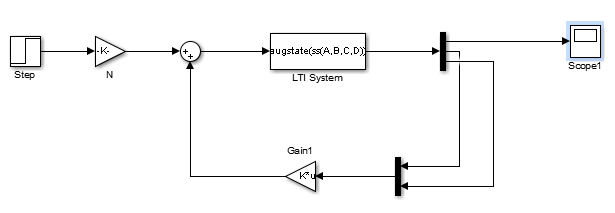
\includegraphics[scale=0.7]{simulink_retourdetat.PNG}
\captionof{figure}{\textit{asservissement par retour d'état.}}
\label{fig1} 
\end{center}












 %Farid
\chapter{COMPARAISON AVEC UN ASSERVISSEMENT AVEC CORRECTION PROPORTIONNELLLE ET RETOUR TACHYMETRIQUE}
\subsection{Retour de sortie avec correcteur proportionnelle}

on considère l'asservissement de position:\\
\begin{center}
$V_m(t)=k_1'(V_r(t)-V_s(t))=k_1'K_e(\theta_r(t)-\frac{K_s}{K_e}\theta_s(t)$
\end{center}
Avec $k_1'$>0 et ici,$K_e=K_s$. il représenter  ci-dessous:
\\


\begin{center}
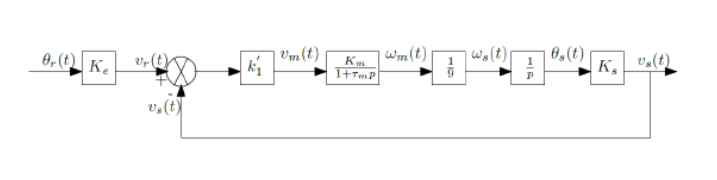
\includegraphics[scale=0.5]{fiiig3.png} 
\captionof{figure}{\textit Asservissement de position avec correction proportionnelle}
\label{fig3}
\end{center}


\subsubsection{Représentation d'état de l'asservissement}
$\omega$=$X_2 et V_s=X_1$

\begin{equation*}
\left\{\begin{matrix}
\dot{x}(t)=Ax(t)+Bu(t)\\ 
y(t)=Cx(t)+Du(t)\\
\end{matrix}\right.
\end{equation*}   


$X_1$=$\frac{K_S}{9p}X_2$\\\\


$X_2$=$\frac{K_mk_1'}{1+Tmp}(V_r-X_1)$\\

\begin{equation*}
\begin{matrix}
\dot{X_1}=\frac{K_s}{9}X_2\\
\dot{X_2}=-\frac{X_2}{T_m}-\frac{K_mk_1'}{T_m}-\frac{K_mk_1'}{Tm}V_r
\end{matrix}
\end{equation*}
\\

L'equation d'etat est:\\\\


$\dot{X}$=$\begin{bmatrix}
0&\frac{K_s}{9}\\
-\frac{K_mk_1'}{T_m}&-\frac{1}{T_m}
\end{bmatrix}X
\quad + \quad
\begin{bmatrix}
0\\
\frac{K_mk_1'}{T_m}
\end{bmatrix}V_r
$

\subsection{Expression de la fonction de transfert}


\begin{center}
$H(p)=\frac{1}{\frac{9T_m}{K_sk_1'K_m}}p^2+\frac{9}{K_sk_1'K_m}p+1$
\end{center}


Le gain statique est 1.
La pulsation naturelle $\omega_n=\sqrt{\frac{K_sk_1'K_m}{9T_m}}$
%L'amortissement $\zeta=\frac{3}{2\sqrt{(T_mK_sK_mk_1')}}$

\subsubsection{Erreur de position $\epsilon_p$}
$\epsilon_p=\lim\limits_{\substack{p \rightarrow 0 }} 1-H(p)$\\
$\epsilon_p=0$

\subsubsection{Erreur de trainage à une rampe $\epsilon_r$}
$\epsilon_r=\lim\limits_{\substack{p \rightarrow 0 }} \frac{1-H(p)}{p}$
$\epsilon_r=2$

Avec la commande MATLAB "rlocus" ce qui nous as permet de  tracer le lieu sur lequel peut  positionner les pôles de l'asservissement voir la figure.



\begin{center}
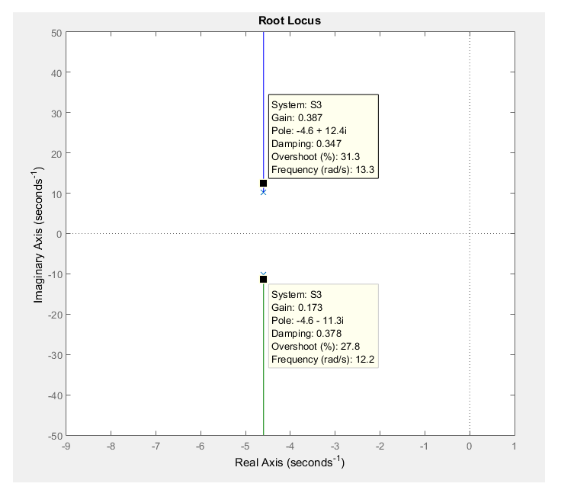
\includegraphics[scale=0.5]{fiiig4.png}
\captionof{figure}{\textit Lieu des pôles de l'asservissement}
\label{fig4} 
\end{center}
 %%******************* Coclusion
\chapter*{Conclusion}
\addcontentsline{toc}{chapter}{Conclusion}

Ce TP nous a permet d'utiliser les différentes commandes de robustesse et a appris de définir un correcteur par étapes, cela en vérifiant chaque contrainte pour déterminer un meilleur correcteur.\\




\begin{appendices}
\chapter*{Annexe 1}
	
				
\end{appendices}





%Bibliographie 
%\bibliographystyle{alpha}
%\bibliography{biblio}




\end{document}







